
%%%%%%%%%%%%%%%%%%%%%%%%%%%%%%%%%%%%%%%%%%%%%%%%%%%%%%%%%%%%%%%%%%%%%%%%%%%%%%%%%%%%%%%
%%%%%%%%%%%%%%%%%%%%%%%%%%%%%%%%%%%%%%%%%%%%%%%%%%%%%%%%%%%%%%%%%%%%%%%%%%%%%%%%%%%%%%%
% 
% This top part of the document is called the 'preamble'.  Modify it with caution!
%
% The real document starts below where it says 'The main document starts here'.

\documentclass[12pt]{article}

\usepackage{amssymb,amsmath,amsthm}
\usepackage[top=1in, bottom=1in, left=1.25in, right=1.25in]{geometry}
\usepackage{fancyhdr}
\usepackage{enumerate}
\usepackage{listings}
\usepackage{graphicx}
\usepackage{float}

\usepackage{mwe}
\usepackage{caption}
\usepackage{subcaption}
% Comment the following line to use TeX's default font of Computer Modern.
\usepackage{times,txfonts}



\makeatletter
\renewcommand*\env@matrix[1][*\c@MaxMatrixCols c]{%
  \hskip -\arraycolsep
  \let\@ifnextchar\new@ifnextchar
  \array{#1}}
\makeatother

\newtheoremstyle{homework}% name of the style to be used
  {18pt}% measure of space to leave above the theorem. E.g.: 3pt
  {12pt}% measure of space to leave below the theorem. E.g.: 3pt
  {}% name of font to use in the body of the theorem
  {}% measure of space to indent
  {\bfseries}% name of head font
  {:}% punctuation between head and body
  {2ex}% space after theorem head; " " = normal interword space
  {}% Manually specify head
\theoremstyle{homework} 

% Set up an Exercise environment and a Solution label.
\newtheorem*{exercisecore}{Exercise \@currentlabel}
\newenvironment{exercise}[1]
{\def\@currentlabel{#1}\exercisecore}
{\endexercisecore}

\newcommand{\localhead}[1]{\par\smallskip\noindent\textbf{#1}\nobreak\\}%
\newcommand\solution{\localhead{Solution:}}

%%%%%%%%%%%%%%%%%%%%%%%%%%%%%%%%%%%%%%%%%%%%%%%%%%%%%%%%%%%%%%%%%%%%%%%%
%
% Stuff for getting the name/document date/title across the header
\makeatletter
\RequirePackage{fancyhdr}
\pagestyle{fancy}
\fancyfoot[C]{\ifnum \value{page} > 1\relax\thepage\fi}
\fancyhead[L]{\ifx\@doclabel\@empty\else\@doclabel\fi}
\fancyhead[C]{\ifx\@docdate\@empty\else\@docdate\fi}
\fancyhead[R]{\ifx\@docauthor\@empty\else\@docauthor\fi}
\headheight 15pt

\def\doclabel#1{\gdef\@doclabel{#1}}
\doclabel{Use {\tt\textbackslash doclabel\{MY LABEL\}}.}
\def\docdate#1{\gdef\@docdate{#1}}
\docdate{Use {\tt\textbackslash docdate\{MY DATE\}}.}
\def\docauthor#1{\gdef\@docauthor{#1}}
\docauthor{Use {\tt\textbackslash docauthor\{MY NAME\}}.}
\makeatother

% Shortcuts for blackboard bold number sets (reals, integers, etc.)
\newcommand{\Reals}{\ensuremath{\mathbb R}}
\newcommand{\Nats}{\ensuremath{\mathbb N}}
\newcommand{\Ints}{\ensuremath{\mathbb Z}}
\newcommand{\Rats}{\ensuremath{\mathbb Q}}
\newcommand{\Cplx}{\ensuremath{\mathbb C}}
%% Some equivalents that some people may prefer.
\let\RR\Reals
\let\NN\Nats
\let\II\Ints
\let\CC\Cplx

%%%%%%%%%%%%%%%%%%%%%%%%%%%%%%%%%%%%%%%%%%%%%%%%%%%%%%%%%%%%%%%%%%%%%%%%%%%%%%%%%%%%%%%
%%%%%%%%%%%%%%%%%%%%%%%%%%%%%%%%%%%%%%%%%%%%%%%%%%%%%%%%%%%%%%%%%%%%%%%%%%%%%%%%%%%%%%%
% 
% The main document start here.

% The following commands set up the material that appears in the header.
\doclabel{STAT 401: Homework 15}
\docauthor{Stefano Fochesatto}
\docdate{\today}


%\begin{figure}[H]
%  \begin{center}
%  \caption{}
%  \includegraphics[\textwidth]{}
%  \end{center}
%\end{figure}

% \textbf{Code:}
% \begin{center}
% \lstinputlisting{}
% \end{center} 



\begin{document}

\begin{exercise}{1} Use the data described in problem 12.1. Do the following:
  \begin{enumerate}
    \item[a.] Create  a table that gives the number of trees that survived and the number that died of each of the nine species.\\
    \solution  The following r script generates the desired table, \\
    \textbf{Code:}
    \begin{center}
    \lstinputlisting{r1.txt}
    \end{center} 
    \newpage

    \item[b.] Create a scatter plot tha puts the proportion of deaths in each species on the y-axis and the logarithm, of average diameter on 
    on the x-axis. You can get the surviving proportion in each species using, \\
    \textbf{aggregate(Blowdown\$y, by=list(Blowdown\$spp),FUN=mean)\$x}\\
    and the average diameter using\\
    \textbf{aggregate(Blowdown\$d, by=list(Blowdown\$spp),FUN=mean)\$x}\\
    Comment on whether the sigmoid curve of logistic regression appears to fit the data in your scatter plot. \\
    \solution Generating the scatterplot we can see that a sigmoid curve might be able to fit the data, with low proportions near the where the 
    log average diameter is in the high 2s and higher proportions in the low 3s. \\
    \begin{figure}[H]
      \begin{center}
      \caption{Scatterplot of Log average diameter vs survival probability.}
      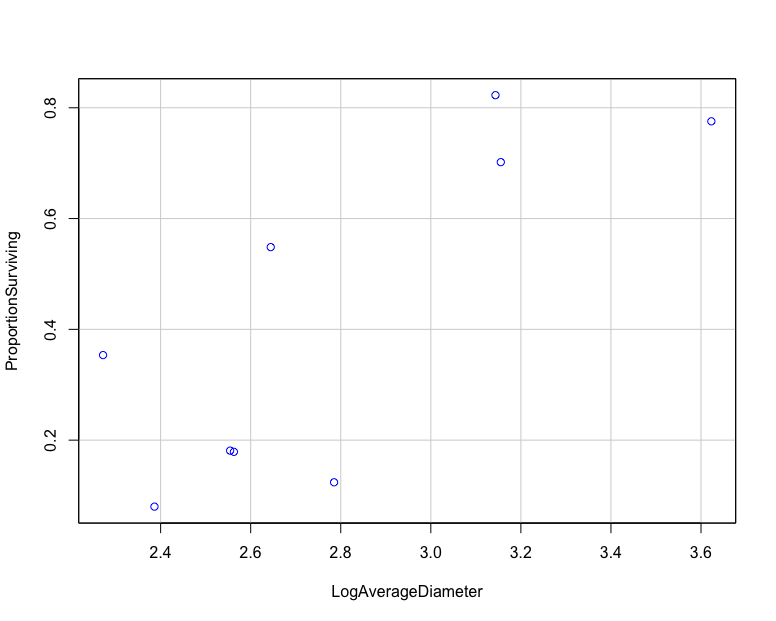
\includegraphics[width = \textwidth]{Rplot01.png}
      \end{center}
    \end{figure}
    \newpage


    \item[c.] Fit the logistic regression model to the raw data using $log(d)$ as the regressor. Draw effects plots of the fitted model.
    \solution  Fitting the logistic regression in r and generating the effects plot we get the following, 
    \begin{figure}[H]
      \begin{center}
      \caption{Plot of Logistic Regression}
      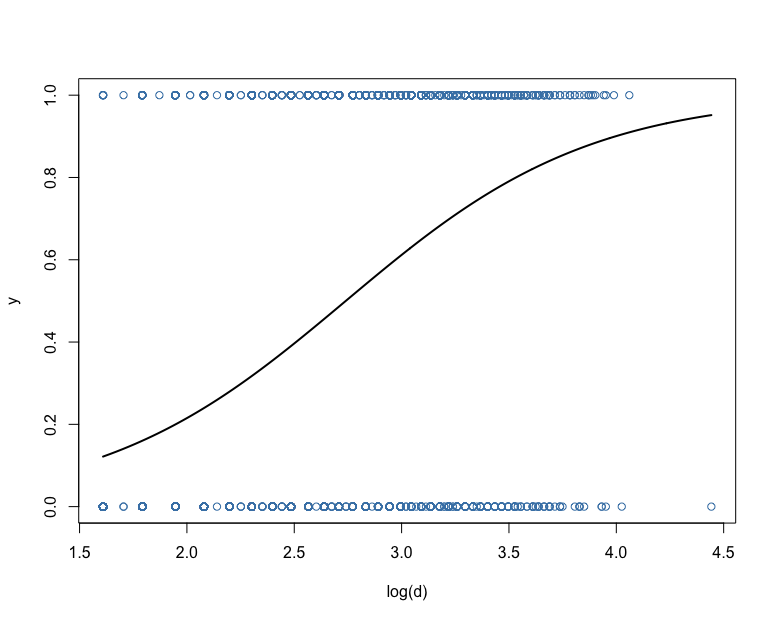
\includegraphics[width = \textwidth]{Rplot.png}
      \end{center}
    \end{figure}
    \begin{figure}[H]
      \begin{center}
      \caption{Effects Plot}
      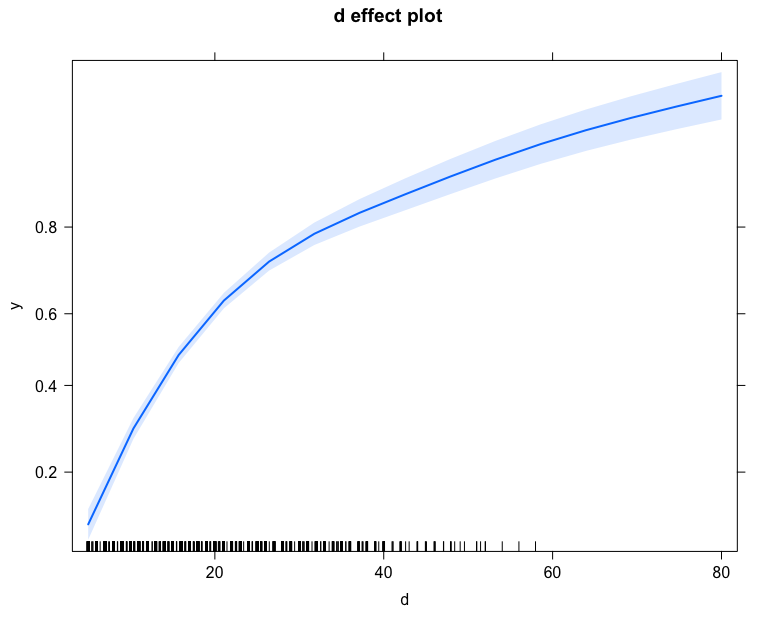
\includegraphics[width = \textwidth]{Rplot02.png}
      \end{center}
    \end{figure}
    \textbf{Code:}
    \begin{center}
    \lstinputlisting[basicstyle = \small]{r2.txt}
    \end{center} 
    \newpage


    \item[d.] Using the fitted model, give an interpretation of the coefficient for log(d)\\
    \solution By looking at the regression summary report we get that as the log of the diameter increases by one unit, the 
    log odds of a tree dying increase by 1.74882. 
    \newpage

    \item[e.] Add $(log(d))^2$ ot the mean funciton form the fitted model to allow for a possible decline in the probabliity of blowdown for the larges trees. Obtain 
    the likelihood ration test for the hypothesis that the quadratic term is 0 and interpret its results. \\
    \solution Fitting the second order model and performing the likelihood ratio test we get p-value on the order of $10^{-14}$ which means that we reject the null hypothesis and conclude that the
    second order is a significant predictor. \\
    \textbf{Code:}
    \begin{center}
    \lstinputlisting[basicstyle = \small]{r3.txt}
    \end{center} 
    \newpage

  \end{enumerate}
\end{exercise}

\begin{exercise}{2} Do problem 12.8. then the problem says 'summarize results', predict the probability of death of a tree with diameter 21cm and local severity measure .5.\\
  \begin{enumerate}
    \item[12.8.1] For the blowdown example, fit the model 
    \begin{equation*}
      y \approx log(d) + s + log(d):s
    \end{equation*} 
    for spp = paper birch and summarize results.\\
    \solution\\
    \textbf{Code:}
    \begin{center}
    \lstinputlisting[basicstyle = \footnotesize]{r4.txt}
    \end{center} 
    \newpage


    \item[12.8.2] Do the same for spp = aspen and summarize results.\\
    \solution \\
    \textbf{Code:}
    \begin{center}
    \lstinputlisting[basicstyle = \footnotesize]{r5.txt}
    \end{center} 
    \newpage

  \end{enumerate}
  
\end{exercise}



\begin{exercise}{3} Use the data described in problem 12.9. Do the following:
  \begin{enumerate}
    \item[a.] Fit a poisson regression model with sex, citizen, and type as predictors and count as the response. interpret the 
    estimated coefficient for each regression.\\
    \solution  Fitting the model in r, we get the following summary report.\\
    \textbf{Code:}
    \begin{center}
    \lstinputlisting[basicstyle = \footnotesize]{r6.txt}
    \end{center}
    Interpreting the coefficients we get that if a subject is male their count changes by a multiplicative factor of $e^{0.73967}$.
    If the subject is a us citizen their count changes by a multiplicative factor of $e^{-0.12885}$. The type coefficients can be interpreted similarly. 
    \newpage

    \item[b.] Perform a goodness-of-fit test on the model using residual deviance. Interpret the test's result. \\
    \solution Computing the p-value for a goodness-of-fit test using residual deviance using r we get a p-value on the order of $10^{-14}$
    so we reject the null hypothesis and conclude that our model does not adequately fit the data. \\
    \textbf{Code:}
    \begin{center}
    \lstinputlisting[basicstyle = \footnotesize]{r7.txt}
    \end{center} 
  \end{enumerate}
  
\end{exercise}



\end{document}





















